%% LyX 1.6.7 created this file.  For more info, see http://www.lyx.org/.
%% Do not edit unless you really know what you are doing.
\author{Andriy Zatserklyaniy, zatserkl@fnal.gov}
\documentclass[english]{article}
\usepackage{amsmath}
%\usepackage{MnSymbol}
\usepackage[T1]{fontenc}
\usepackage[latin9]{inputenc}
\usepackage{graphicx}
% \usepackage[pdftex]{graphicx}
\usepackage{esint}
\usepackage{babel}
\usepackage{parskip}            % for \smallskip, \medskip and \bigskip

\usepackage{cancel}             % to cancel out variables in text

\usepackage[active]{srcltx}     % to load source file from dvi

\usepackage{epstopdf}           % creates pdf files from eps adding to filename -eps-converted-to

%\usepackage{epsfig}             % I used it all the time. Considered obsolete now.
%\usepackage[normalem]{ulem}
%\usepackage{arcs}

%-- function to scale pictures --%
\makeatletter
\def\ScaleIfNeeded{%
\ifdim\Gin@nat@width>\linewidth
\linewidth
\else
\Gin@nat@width
\fi
}

\begin{document}

\title{Pulse function}

\maketitle

\section{Derive the function}

%-- page 1s

Define the function as a charging/discharging of capacitor. 
To take into account finite width of light pulse and clipping capacitor\cite{bib:NIM April 2010} we parametrize the pulse function by two time constants: rise time $\tau_1$ and discharge time $\tau_2$.

\begin{equation}
p(t)=(1-e^{-t/\tau_1})e^{-t/\tau_2}, \quad t>0
\end{equation}

\begin{figure}[h]
\centering
\begin{minipage}[t]{0.75 \linewidth}
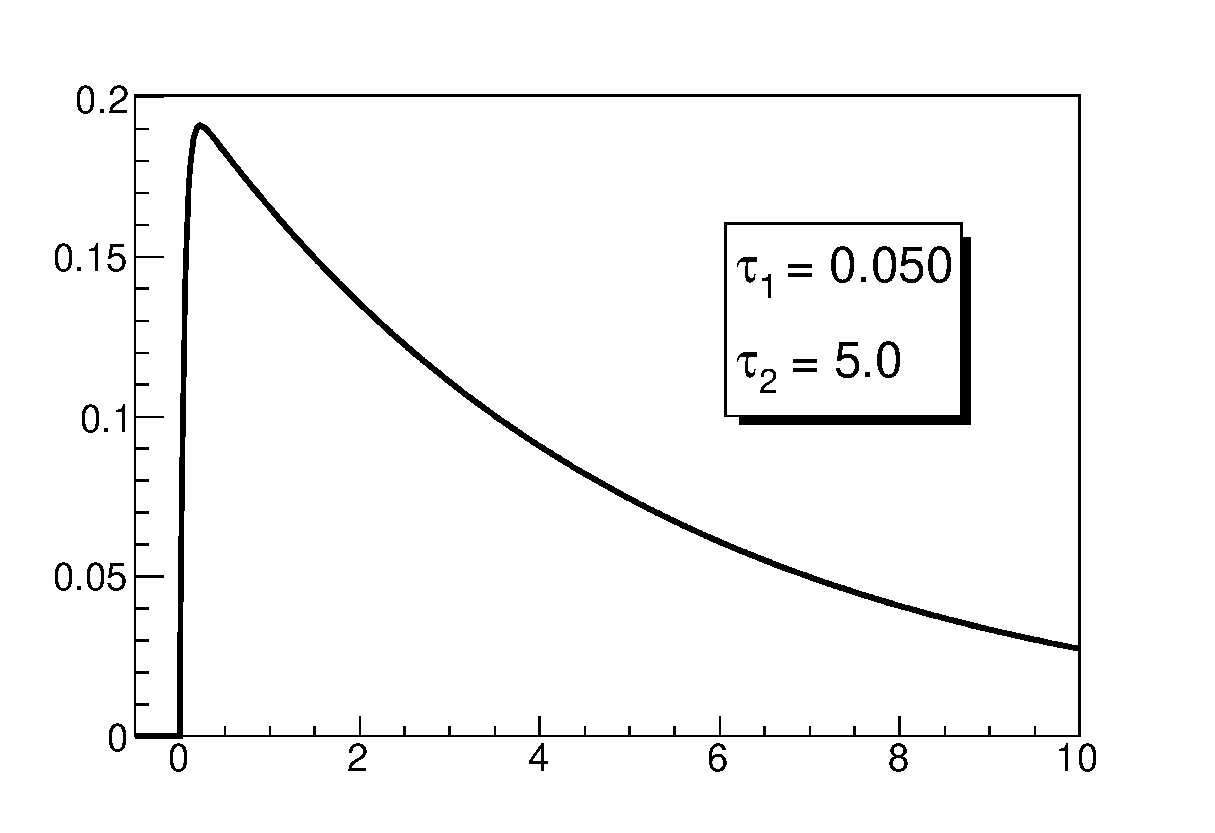
\includegraphics[width=\ScaleIfNeeded]{pulse.eps}   % TF1* erf = new TF1("erf", "TMath::Erf(x)", -3,3); erf->SetTitle("")
% \caption{Pulse function $p(x)=\frac{\tau_1+\tau_2}{\tau_2^2}(1-e^{-x/\tau_1})e^{-x/\tau_2}$}\label{fig:p}
\caption{Pulse function.}\label{fig:pulse}
\end{minipage}
\end{figure}

The pulse function is defined on $(0, +\infty)$. Normalize it to 1.
\begin{align*}
& \int_{0}^{\infty}(1-e^{-x/\tau_1})e^{-x/\tau_2}dx = \\
& \int_{0}^{\infty}e^{-x/\tau_2}dx - \int_{0}^{\infty}e^{-x/\tau_1}e^{-x/\tau_2}dx =\\
& \tau_2 + \dfrac{1}{\frac{1}{\tau_1}+\frac{1}{\tau_2}} = \dfrac{\tau_2^2}{\tau_1+\tau_2}
\end{align*}

Write pulse function normalized with factor A as

\begin{equation}
p(x) = A \dfrac{\tau_1+\tau_2}{\tau_2^2} (1-e^{-x/\tau_1})e^{-x/\tau_2}
\end{equation}

Fig.\ref{fig:pulse} shows normalized pulse function for $A=1$, $\tau_1=0.050$ and $\tau_2=1$.

Because $ \int_0^\infty p(t)dt = A $

$ [A] = QR $

$ [p(x)] = [R]\dfrac{[Q]}{[t]} = [R][I] = [V] = $ Volts

%-- page 2s

\section{Convolution with scintillator decay}

Let's assume that scintillator decay time is $T$ and normalize scintillator decay function $s(t)$ to 1:

\begin{align*}
\int_0^\infty s(t)dt = 1, \quad \int_0^\infty e^{-t/T}dt = T
\end{align*}

so

\begin{equation}
s(t) = \dfrac{1}{T} e^{-t/T}
\end{equation}

Convolute pulse function with scintillator decay

\begin{equation}
P(x) = \int_0^x s(t)p(x-t)dt
\end{equation}

In general case with integration limits $a$ and $b$

\begin{align*}
P(x) & = \int_a^b s(t)p(x-t)dt = \left\lvert
        \begin{aligned}
        & z = x-t & dz = -dt \\
        & t = a   & z = x-a \\
        & t = b   & z = x-b
        \end{aligned}
\right\rvert
\quad = -\int_{x-a}^{x-b} s(x-z)p(z)dz \\
& = \int_{x-b}^{x-a} s(x-z)p(z)dz
\end{align*}

Because in our case $a=0$ and $b=x$

%-- works fine
% \begin{align}
% P(x) & = \nonumber \\
% & \int_a^b s(t)p(x-t)dt \nonumber \\
% & \int_a^b s(t-x)p(t)dt
% \end{align}

\begin{equation}\label{conv_with_scint}
\boxed{ P(x) = \int_0^x s(t-x)p(t)dt }
\end{equation}

We will use Eq\eqref{conv_with_scint} for $P(x)$ for following calculations.

\begin{align*}
P(x) & = A \frac{\tau_1+\tau_2}{\tau_2^2} \frac{1}{T} 
\int_0^x e^{-\frac{x-t}{T}} (1-e^{-t/\tau_1}) e^{-t/\tau_2} dt \\
& =  A\frac{\tau_1+\tau_2}{\tau_2^2}\frac{1}{T} e^{-\frac{x}{T}}
\Bigl[
\int_0^x e^{ -(\frac{1}{\tau_2}-\frac{1}{T})t } dt 
- 
\int_0^x e^{ -(\frac{1}{\tau_1}+\frac{1}{\tau_2}-\frac{1}{T})t } dt
\Bigr] \\
%
& =  A\frac{\tau_1+\tau_2}{\tau_2^2}\frac{1}{T} e^{-\frac{x}{T}}
\Bigl[
\int_0^x e^{ -(\frac{1}{\tau_2}-\frac{1}{T})t } dt 
- 
\int_0^x e^{ -(\frac{1}{\tau_{12}}-\frac{1}{T})t } dt
\Bigr]
\end{align*}
%
where
\begin{equation} \boxed{ \tau_{12} = \frac{\tau_1\tau_2}{\tau_1 + \tau_2} } \end{equation}
%
\begin{align*}
% P(x) & =  A\frac{\tau_1+\tau_2}{\tau_2^2}\frac{1}{T} e^{-x/T}
P(x) & =  A\frac{\tau_1+\tau_2}{\tau_2^2}\frac{1}{T} e^{-\frac{x}{T}}
\Bigl[
\frac{-1}{\frac{1}{\tau_2}-\frac{1}{T}} \left( e^{ -(\frac{1}{\tau_2}-\frac{1}{T})x} - 1 \right) -
\frac{-1}{\frac{1}{\tau_{12}}-\frac{1}{T}} \left( e^{ -(\frac{1}{\tau_{12}}-\frac{1}{T})x} - 1 \right)
\Bigr] \\
%
& = A\frac{\tau_1+\tau_2}{\tau_2^2} e^{-\frac{x}{T}}
\Bigl[
\frac{-\tau_2}{T-\tau_2} \left( e^{ -(\frac{1}{\tau_2}-\frac{1}{T})x} - 1 \right) -
\frac{-\tau_{12}}{T-\tau_{12}} \left( e^{ -(\frac{1}{\tau_{12}}-\frac{1}{T})x} - 1 \right)
\Bigr] \\
%
& = A\frac{\tau_1+\tau_2}{\tau_2^2} e^{-\frac{x}{T}}
\Bigl[
\frac{\tau_2}{T-\tau_2} \left( 1 - e^{ -(\frac{1}{\tau_2}-\frac{1}{T})x} \right) -
\frac{\tau_{12}}{T-\tau_{12}} \left( 1 - e^{ -(\frac{1}{\tau_{12}}-\frac{1}{T})x} \right)
\Bigr] \\
%
& = A\frac{\tau_1+\tau_2}{\tau_2^2}
\Bigl[
\frac{\tau_2}{T-\tau_2} \left( e^{-\frac{x}{T}} - e^{-\frac{x}{\tau_2}} \right) -
\frac{\tau_{12}}{T-\tau_{12}} \left( e^{-\frac{x}{T}} - e^{-\frac{x}{\tau_{12}}} \right)
\Bigr]
\end{align*}
%
% \begin{align*}
% P(x) & =  A \dfrac{\tau_1+\tau_2}{\tau_2^2} \dfrac{1}{\cancel{T}}
% \Bigl[
% \dfrac{\cancel{T}\tau_2}{T-\tau_2} (e^{-x/T} - e^{-x/\tau_2}) - 
% \dfrac{\cancel{T}\tau_{12}}{T-\tau_{12}} (e^{-x/T} - e^{-x/\tau_{12}})
% \Bigr] \\
% \end{align*}
%
\begin{align}
P(x) & =  A \dfrac{\tau_1+\tau_2}{\tau_2^2} 
\Bigl(
\tau_2 \dfrac{e^{-x/T} - e^{-x/\tau_2}}{T-\tau_2} -
\tau_{12} \dfrac{e^{-x/T} - e^{-x/\tau_{12}}}{T-\tau_{12}} 
\Bigr) \label{eq:Pscint}
\end{align}
Define 
\begin{equation}\label{eq:ITtau} \boxed{
  I_{T\tau} = \tau \dfrac{e^{-x/T} - e^{-x/\tau}}{T-\tau}
} \end{equation}
then 
\begin{equation} \boxed{ 
  P(x) = A \dfrac{\tau_1 + \tau_2}{\tau_2^2} \Bigl( I_{T\tau_2}(x) - I_{T\tau_{12}}(x) \Bigr)
}
\end{equation}

Fig.\ref{fig:Pscint} shows result of convolution function from Fig.\ref{fig:pulse} with scintillator decay function with decay time $T=40$.
Note on shift of the maximum from about 0 to about 10.
Using Eq\eqref{eq:Pscint} we can estimate shift of the maximum for the function plotted on Fig.\ref{fig:Pscint}. 
Because $\tau_1 << \tau_2$ we can neglect the second term in parenthesis. If we equate to 0 derivative of the first term we will find
\begin{align*}
\frac{1}{T} e^{-x/T} - \frac{1}{\tau_2} e^{-x/\tau_2} = 0 \\
\frac{1}{T} - \frac{1}{\tau_2} e^{-\left(\frac{1}{\tau_2}-\frac{1}{T}\right)x} = 0 \\
e^{-(\frac{1}{\tau_2} - \frac{1}{T})x} = \frac{\tau_2}{T} \\
-\left( \frac{1}{\tau_2} - \frac{1}{T} \right) x = ln\frac{\tau_2}{T} \\
= \frac{T\tau_2}{T-\tau_2} ln\frac{T}{\tau_2} \\
\text{because of } T >>\tau_2 \\
x \approx \tau_2 ln\frac{T}{\tau_2}
\end{align*}
%
In numbers \\
% $x \approx 1 \cdot ln \frac{40}{1} \approx 3.7$
$$
x \approx 5 \cdot ln \frac{40}{5} \approx 10
$$

\begin{figure}[h]
\centering
\begin{minipage}[t]{0.75 \linewidth}
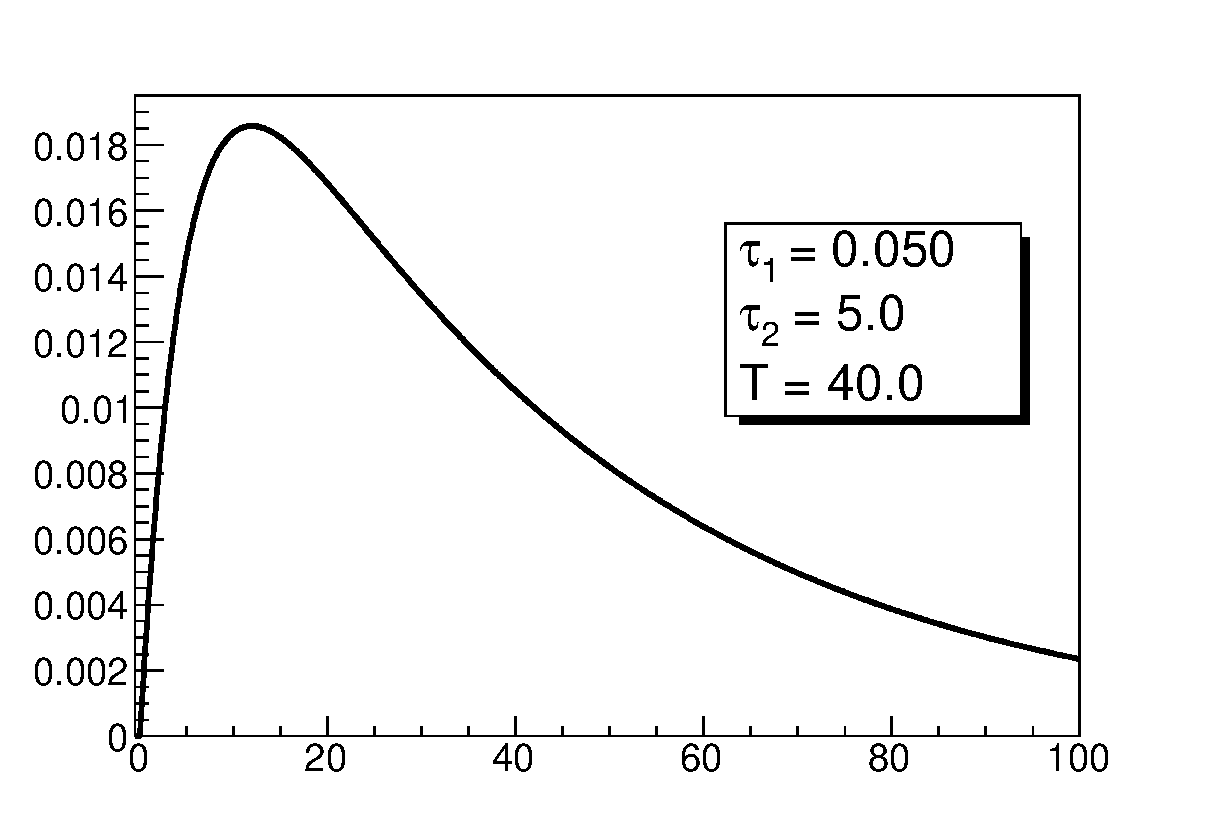
\includegraphics[width=\ScaleIfNeeded]{Pscint.eps}
\caption{Convolution with scintillator decay function.}\label{fig:Pscint}
\end{minipage}
\end{figure}

%-- page 4s

\section{Special cases}

NB: $\tau_2$ is always finite while $\tau_1$ and $T$ can be 0.
In function $I_{T\tau}$ $\tau$ can be $\tau_1$ or $\tau_{12}$; $\tau_{12}$ can be 0 when $\tau_1=0$.

Expression \eqref{eq:ITtau} will blow up during computing at $T \to \tau$. Except that it worth to consider cases $\tau \to 0$ and $T \to 0$. 
% What if $\tau$ and $T$ will go to 0 at the same time?

{\bf Case 1} \hspace{1cm} $\boxed{\tau \to 0}$ 
\hspace{1cm} $I_{T\tau} \to 0$ \hspace{1cm} $I_{T\tau} = 0$

Assume that $\tau > \epsilon$ now.

{\bf Case 2} \hspace{1cm} $\boxed{T \to 0}$
\hspace{1cm} $I_{T\tau} = e^{-x/\tau}$

Assume that both $\tau > \epsilon$ and $T > \epsilon$ now.

{\bf Case 3} \hspace{1cm} $\boxed{\tau \to T}$ \ % backslash followed by space to insert line break
\begin{align*}
I_{T\tau} & = \tau \frac{e^{-x/T} - e^{-x/\tau}}{T-\tau} = 
\tau e^{-x/\tau} \frac{e^{ (\frac{1}{\tau}-\frac{1}{T})x}-1}{T-\tau} \\ 
& \underset{\tau \to T}{\longrightarrow} \quad
\tau e^{-x/\tau} \frac{\frac{1}{\tau} - \frac{1}{T}}{T-\tau} x \quad
\underset{\tau \to T}{\longrightarrow} \quad \cancel{\tau} e^{-x/\tau} \dfrac{x}{T\cancel{\tau}}
= \frac{x}{T} e^{-x/\tau} \\
& = \frac{x}{\tau} e^{-x/\tau}
\end{align*}

%-- page 5s

\section{Smearing with resolution function}

To take into account signal jitter we convolute pulse function with resolution function: Gaussian with width $\sigma$

\begin{equation}
G(t) = \dfrac{1}{\sqrt{2\pi}\sigma} e^{-\frac{t^2}{2\sigma^2}}
\end{equation}

Convolution integral runs from $-\infty$ to $\infty$.
\begin{equation}
{\cal P}_\sigma (x) = \int_{-\infty}^\infty dt P(t) G(t-x) = 
\dfrac{1}{\sqrt{2\pi}\sigma} \int_{-\infty}^\infty P(t) e^{-\frac{(t-x)^2}{2\sigma^2}} dt
\end{equation}

Take into account that $P(t)=0$ for $t<0$

then

\begin{equation}
{\cal P}_\sigma (x) = 
\dfrac{1}{\sqrt{2\pi}\sigma} \int_0^\infty P(t) e^{-\frac{(t-x)^2}{2\sigma^2}} dt
\end{equation}

We can also use a step function 
\begin{equation*}
e(x) =
\begin{cases}
1 & \text{if } x \geq 0 \\
0 & \text{if } x < 0
\end{cases}
\end{equation*}
to extend integration to $-\infty$. The total area under smeared pulse function should be equal to area under unsmeared function: 
\begin{align*}
\int_{-\infty}^\infty {\cal P}_\sigma (x) dx = 
\int_{-\infty}^\infty dx \int_{-\infty}^\infty P(t) e(t) G(t-x) dt = \\
\int_{-\infty}^\infty dt P(t) e(t) \underbrace{\int_{-\infty}^\infty G(t-x) dx}_{= 1} = %-- works
\int_{-\infty}^\infty P(x) dx
\end{align*}

The smearing does not introduce new special cases except $\sigma=0$, therefore we will smear special cases separately. 

In general case
\begin{equation*}
{\cal P}_\sigma(x) = A \frac{\tau_1+\tau_2}{\tau_2^2} 
\Bigl(
\frac{1}{\sqrt{2\pi}\sigma} \int_0^\infty I_{T\tau_2}(t)    e^{-\frac{(t-x)^2}{2\sigma^2}}dt -
\frac{1}{\sqrt{2\pi}\sigma} \int_0^\infty I_{T\tau_{12}}(t) e^{-\frac{(t-x)^2}{2\sigma^2}}dt 
\Bigr)
\end{equation*}
Denote
\begin{equation} \boxed{
  I_{T\tau}^\sigma = \frac{1}{\sqrt{2\pi}\sigma} \int_0^\infty I_{T\tau}(t)e^{-\frac{(t-x)^2}{2\sigma^2}}dt
}
\end{equation}
Here $\tau$ can serve as $\tau_1$ or $\tau_{12}$. Then 
\begin{equation} \boxed{
  {\cal P}_\sigma(x) = A \frac{\tau_1+\tau_2}{\tau_2^2} 
  \Bigl(
  I_{T\tau_2}^\sigma (x) - I_{T\tau_{12}}^\sigma (x)
  \Bigr)
}
\label{eq:Psigma}
\end{equation}

\begin{align}
I_{T\tau}^\sigma(x) & = \frac{1}{\sqrt{2\pi}\sigma} \dfrac{\tau}{T-\tau}
\Bigl(
\int_0^\infty e^{-t/T}    e^{-\frac{(t-x)^2}{2\sigma^2}} dt - 
\int_0^\infty e^{-t/\tau} e^{-\frac{(t-x)^2}{2\sigma^2}} dt
\Bigr) \nonumber \\ 
%
& = \frac{\tau}{T-\tau} 
\Bigl(
\frac{1}{\sqrt{2\pi}\sigma} \int_0^\infty e^{-t/T}    e^{-\frac{(t-x)^2}{2\sigma^2}} dt - 
\frac{1}{\sqrt{2\pi}\sigma} \int_0^\infty e^{-t/\tau} e^{-\frac{(t-x)^2}{2\sigma^2}} dt 
\Bigr) \label{eq:ITtausigma}
\end{align}
If we denote
% \begin{equation}
% I_\tau^\sigma(x) = \frac{1}{\sqrt{2\pi}\sigma} \int_0^\infty e^{-t/\tau} e^{-\frac{(t-x)^2}{2\sigma^2}} dt
% \label{eq:Itausigma}
% \end{equation}
%-- use {\cal T} instead of \tau
\begin{equation}
I_{\cal T}^\sigma(x) = \frac{1}{\sqrt{2\pi}\sigma} \int_0^\infty e^{-t/{\cal T}} e^{-\frac{(t-x)^2}{2\sigma^2}} dt
\label{eq:Itausigma}
\end{equation}
we can write Eq\eqref{eq:ITtausigma} as
%
\begin{equation}
I_{T\tau}^\sigma(x) = \frac{\tau}{T-\tau} ( I_T^\sigma(x) - I_\tau^\sigma(x) )
\label{eq:ITtausigma_Itausogma}
\end{equation}
%
To calculate integral $I_{\cal T}^\sigma(x)$ Eq\eqref{eq:Itausigma} rewrite
\begin{equation}
e^{ -\frac{t}{{\cal T}}} e^{-\frac{(t-x)^2}{2\sigma^2} } = 
e^{-\frac{x}{{\cal T}}} e^{ \frac{\sigma^2}{2{\cal T}^2} }
e^{ -(\frac{t}{\sigma\sqrt{2}} - \frac{x-\sigma^2/{\cal T}}{\sigma\sqrt{2}})^2 }
\end{equation}
then
\begin{align*}
I_{\cal T}^\sigma(x) & = \frac{1}{\sqrt{2\pi}\sigma} e^{-\frac{x}{{\cal T}}} e^{ \frac{\sigma^2}{2{\cal T}^2} } 
\int_0^\infty e^{ -(\frac{t}{\sigma\sqrt{2}} - \frac{x-\sigma^2/{\cal T}}{\sigma\sqrt{2}})^2 } dt \\
%
& = \frac{1}{\sqrt{2\pi}\sigma} e^{-\frac{x}{{\cal T}}} e^{ \frac{\sigma^2}{2{\cal T}^2} } \sigma\sqrt{2} 
\int_0^\infty e^{ -(\frac{t}{\sigma\sqrt{2}} - \frac{x-\sigma^2/{\cal T}}{\sigma\sqrt{2}})^2 } 
\frac{dt}{\sigma\sqrt{2}} \\
\end{align*}
%
Use substitution
%
\begin{align*}
& z = \frac{t}{\sigma\sqrt{2}}
&& u = z-\frac{x-\sigma^2/{\cal T}}{\sigma\sqrt{2}} \\      %--NB two ampersands: &&
%
& z = 0
&& u = -\frac{x-\sigma^2/{\cal T}}{\sigma\sqrt{2}}
\end{align*}
%
then
%
\begin{align*}
I_{\cal T}^\sigma(x) & =
\frac{1}{\sqrt{2\pi}\sigma} e^{-\frac{x}{{\cal T}}} e^{ \frac{\sigma^2}{2{\cal T}^2} } \sigma\sqrt{2}
\int_{-\frac{x-\sigma^2/{\cal T}}{\sigma\sqrt{2}}}^\infty e^{-u^2} du \\
& = \frac{1}{\sqrt{2\pi}\sigma} e^{-\frac{x}{{\cal T}}} e^{ \frac{\sigma^2}{2{\cal T}^2} } \sigma\sqrt{2}
\cdot \frac{\sqrt{\pi}}{2} \cdot
\frac{2}{\sqrt{\pi}} \int_{-\frac{x-\sigma^2/{\cal T}}{\sigma\sqrt{2}}}^\infty e^{-u^2} du \\
& = \frac{1}{2} e^{-\frac{x}{{\cal T}}} e^{\frac{\sigma^2}{2{\cal T}^2}} \cdot
\frac{2}{\sqrt{\pi}} \int_{-\frac{x-\sigma^2/{\cal T}}{\sigma\sqrt{2}}}^\infty e^{-u^2} du
\end{align*}
%
A complementary error function $erfc(x)$ is defined as $erfc(x) = 1 - erf(x)$, where $erf(x)$ is error function
\begin{equation}
erf(x) = \frac{2}{\sqrt{\pi}} \int_0^x e^{-u^2} du
\end{equation}

The complementary error function can be also written in form 

\begin{equation}
erfc(x) = \frac{2}{\sqrt{\pi}} \int_x^\infty e^{-u^2} du
\end{equation}

% (See plot on page~\pageref{fig:erfc}) \\
See plots on Fig.~\ref{fig:erf} and Fig.~\ref{fig:erfc}. Note that $erfc(x)$ is always positive and $erfc(-\infty) = 2$.

% \begin{figure}
% \centering
% 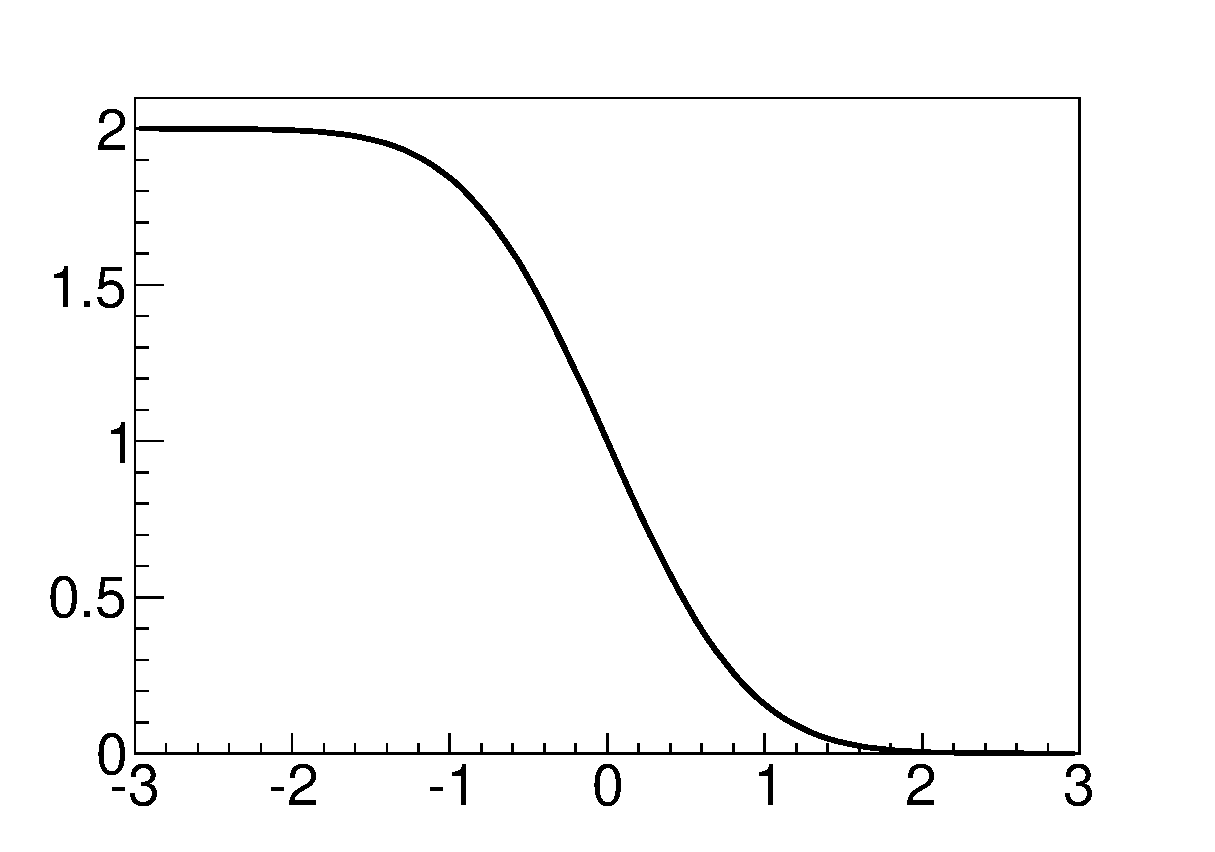
\includegraphics[scale=0.5]{erfc.eps}   % TF1* erfc = new TF1("erfc", "TMath::Erfc(x)", -3,3); erfc->SetTitle("")
% \caption{Complementary Error Function $erfc(x)$}\label{fig erfc}    % NB: label should follow caption
% \end{figure}

%
% Traditional way with given scale factor
%
% \begin{figure}
% \begin{minipage}[t]{0.48 \linewidth}
% \centering
% 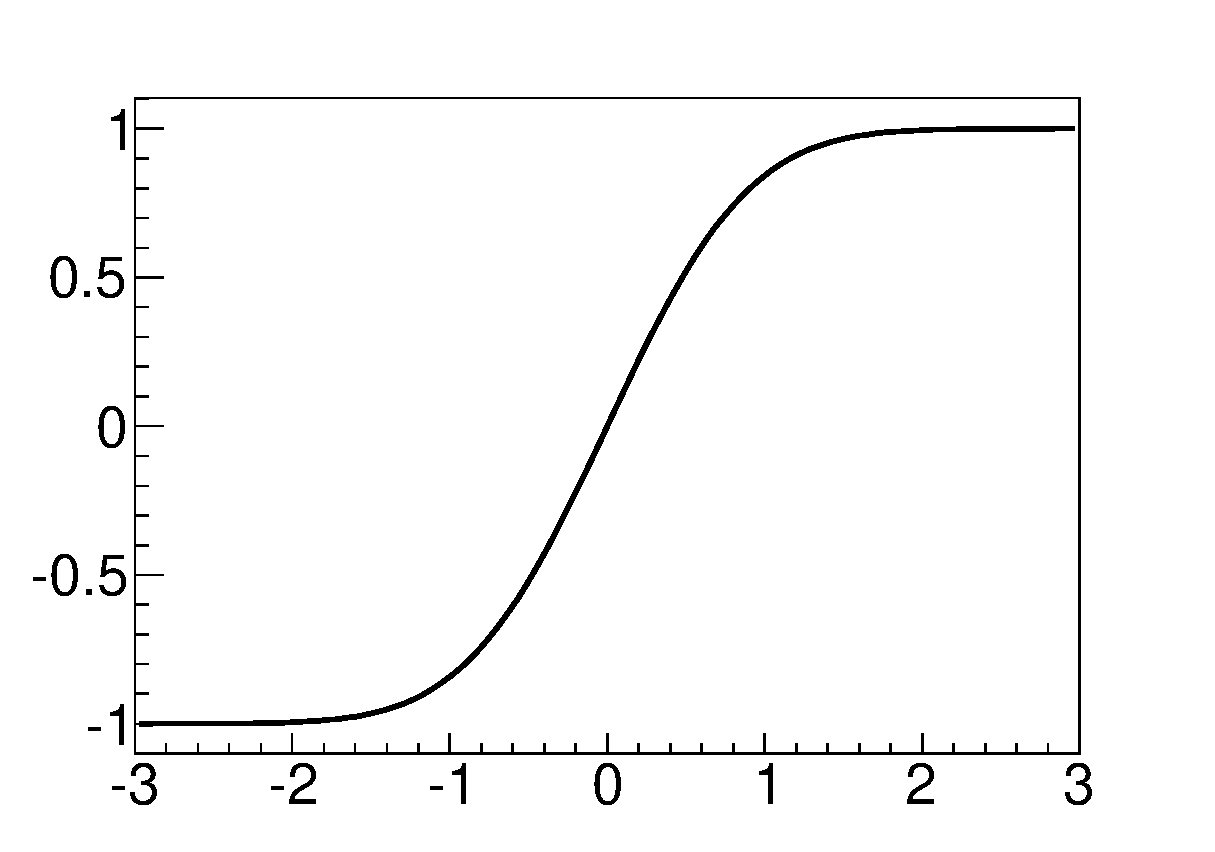
\includegraphics[scale=0.25]{erf.eps}   % TF1* erf = new TF1("erf", "TMath::Erf(x)", -3,3); erf->SetTitle("")
% \caption{Error function $erf(x)$}\label{fig erf}    % NB: label should follow caption
% \end{minipage}
% % \hspace{0.5cm}                          % hspace to separate figures
% \begin{minipage}[t]{0.48 \linewidth}
% \centering
% 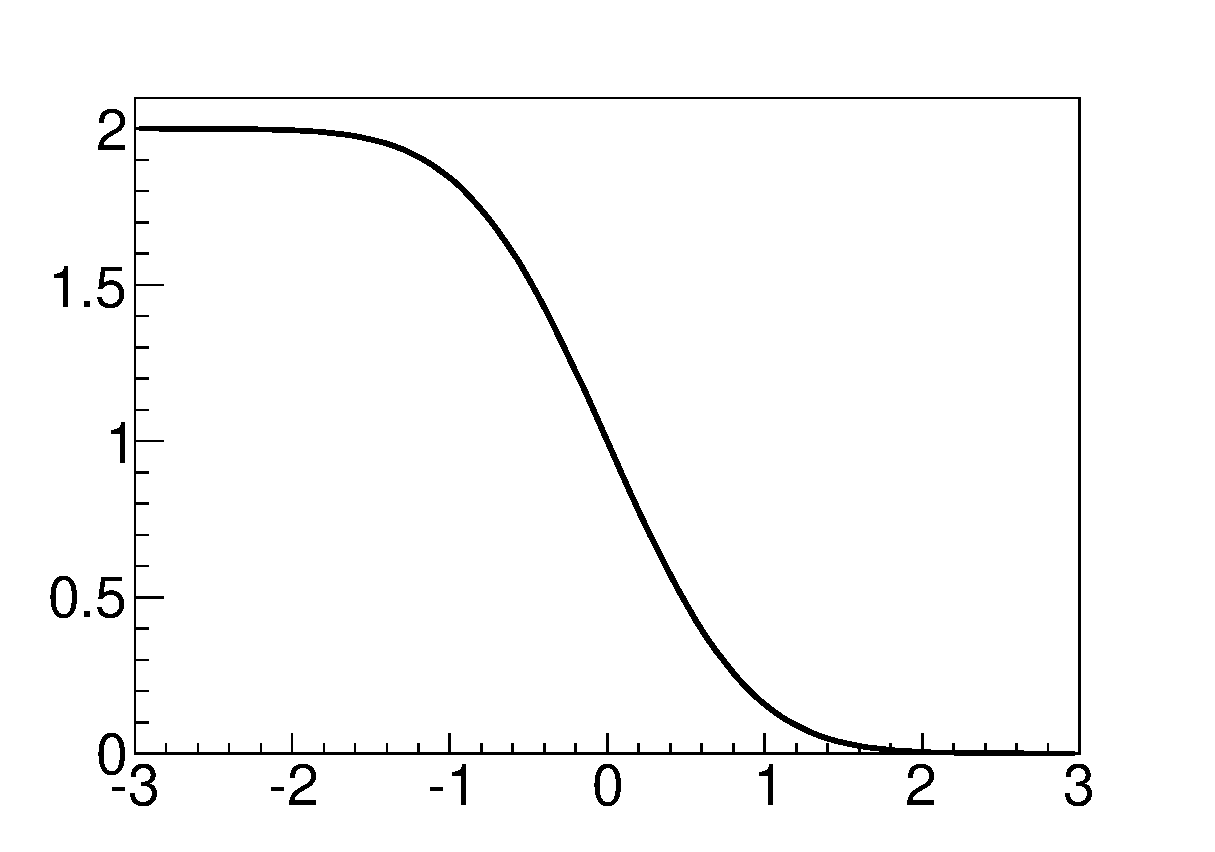
\includegraphics[scale=0.25]{erfc.eps}   % TF1* erfc = new TF1("erfc", "TMath::Erfc(x)", -3,3); erfc->SetTitle("")
% \caption{Complementary error function $erfc(x)$}\label{fig erfc}    % NB: label should follow caption
% \end{minipage}
% \end{figure}

%
% automatic scaling using function ScaleIfNeeded defined after includes before begin{document}
%
% \makeatletter
% \def\ScaleIfNeeded{%
% \ifdim\Gin@nat@width>\linewidth
% \linewidth
% \else
% \Gin@nat@width
% \fi
% }
%
\begin{figure}[ht]
\begin{minipage}[t]{0.48 \linewidth}
\centering
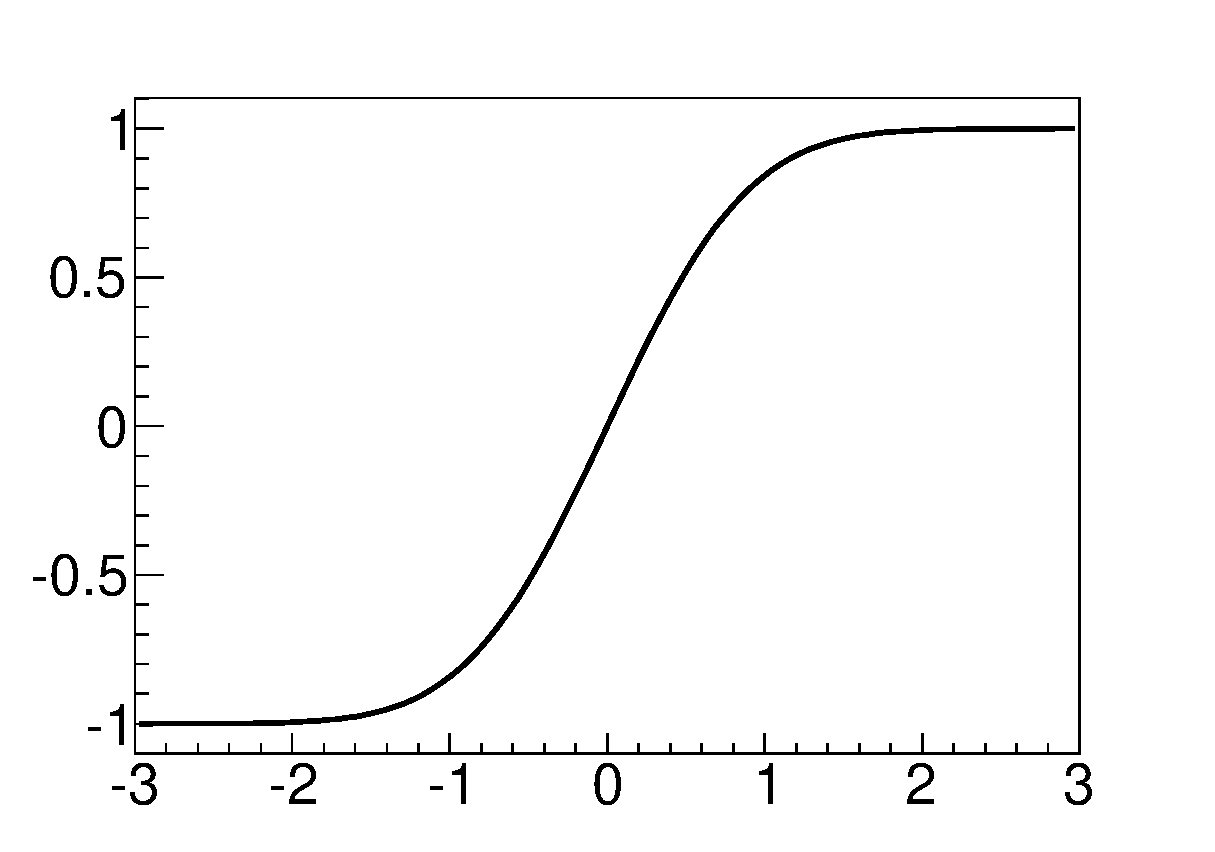
\includegraphics[width=\ScaleIfNeeded]{erf.eps}   % TF1* erf = new TF1("erf", "TMath::Erf(x)", -3,3); erf->SetTitle("")
\caption{Error function $erf(x)$}\label{fig:erf}    % NB: label should follow caption
\end{minipage}
% \hspace{0.5cm}                          % hspace to separate figures
\begin{minipage}[t]{0.48 \linewidth}
\centering
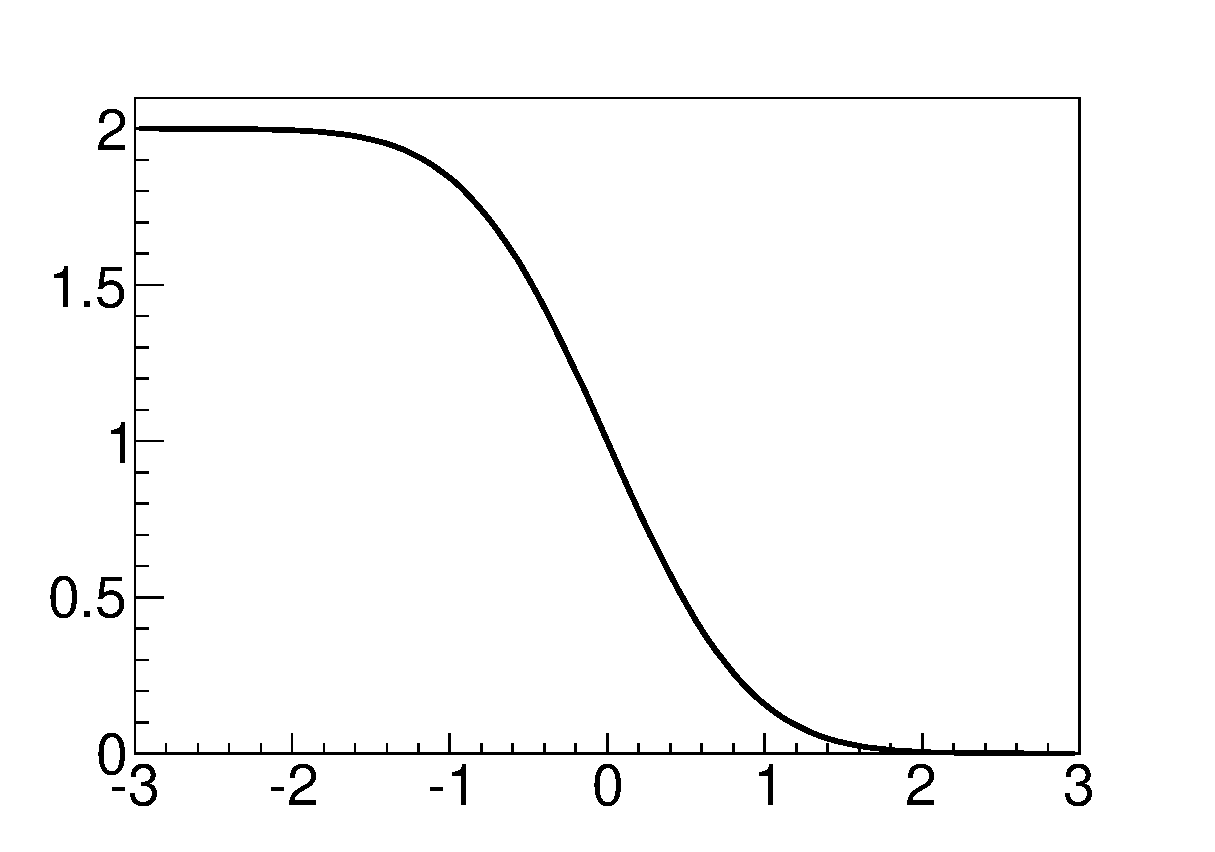
\includegraphics[width=\ScaleIfNeeded]{erfc.eps}   % TF1* erfc = new TF1("erfc", "TMath::Erfc(x)", -3,3); erfc->SetTitle("")
\caption{Complementary error function $erfc(x)$}\label{fig:erfc}    % NB: label should follow caption
\end{minipage}
\end{figure}
%
In terms of $erfc(x)$ 
%
\begin{align}
I_{\cal T}^\sigma(x) & =
\frac{1}{2} e^{-\frac{x}{{\cal T}}} e^{\frac{\sigma^2}{2{\cal T}^2}} erfc(-\frac{x-\sigma^2/{\cal T}}{\sigma\sqrt{2}})
\end{align}
%
Now the Eq\eqref{eq:ITtausigma_Itausogma} becomes
%
\begin{equation}
I_{T\tau}^\sigma(x) = \frac{\tau}{T-\tau}
\left(
\frac{1}{2} e^{-\frac{x}{T}} e^{\frac{\sigma^2}{2T^2}} erfc(-\frac{x-\sigma^2/T}{\sigma\sqrt{2}}) -
\frac{1}{2} e^{-\frac{x}{\tau}} e^{\frac{\sigma^2}{2\tau^2}} erfc(-\frac{x-\sigma^2/\tau}{\sigma\sqrt{2}})
\right)
\label{eq:ITtausigma_Itausogma_new}
\end{equation}
This expression is need to be plugged in Eq\eqref{eq:Psigma}.

Fig.\ref{fig:Psigma} shows an example of pulse function convoluted with scintillator decay and resolution functions. 

\begin{figure}[h]
\centering
\begin{minipage}[t]{0.75 \linewidth}
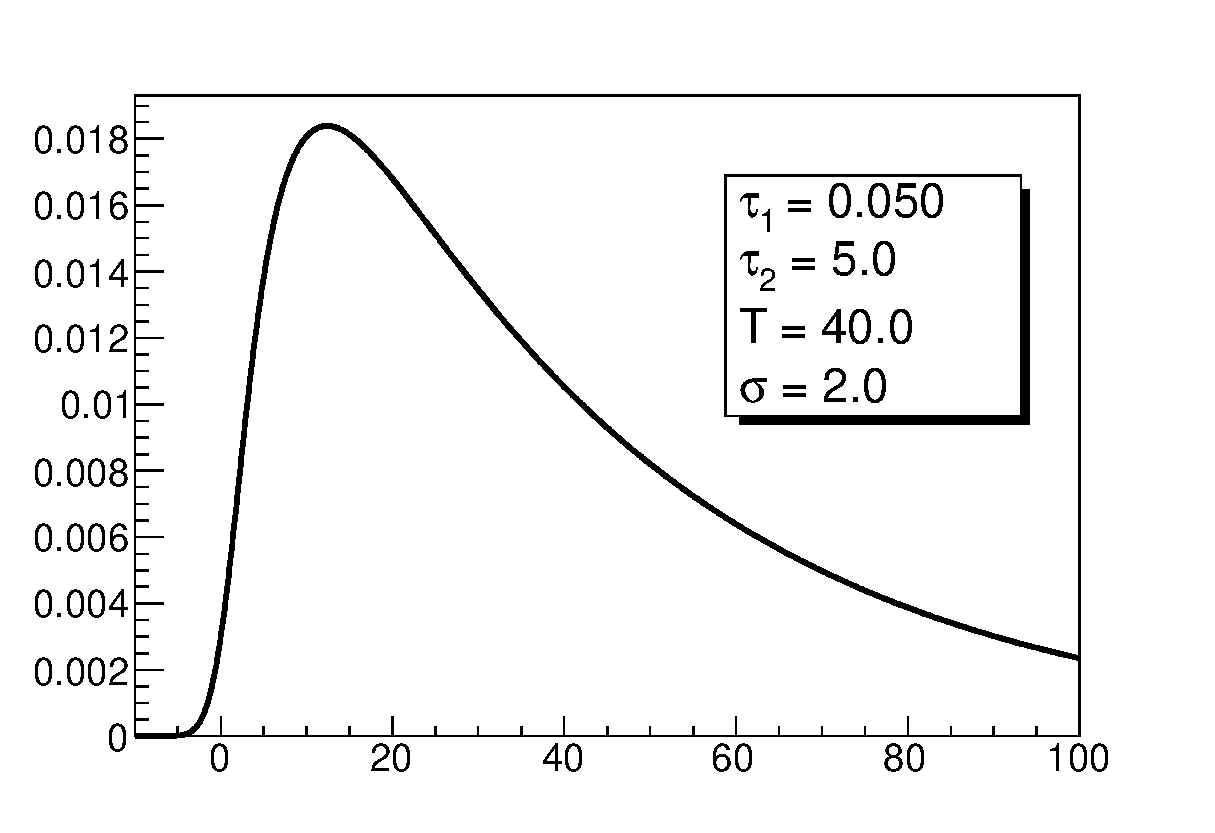
\includegraphics[width=\ScaleIfNeeded]{Psigma.eps}
\caption{Convolution with scintillator decay and resolution functions.}\label{fig:Psigma}
\end{minipage}
\end{figure}

%-------------- page 8s -----------------

\subsection{Smearing in special cases}

{\bf Case 1} \hspace{1cm} $\boxed{\tau_1 \to 0}$ \hspace{1cm}
$I_{T\tau} \to 0 \Rightarrow I_{T\tau}^\sigma = 0$

Assume that $\tau > \epsilon$ now.

{\bf Case 2} \hspace{1cm} $\boxed{T \to 0}$ \hspace{1cm} 
$
I_{T\tau} = e^{-x/\tau} \Rightarrow 
I_{T\tau}^\sigma = 
\frac{1}{2} e^{-\frac{x}{\tau}} e^{\frac{\sigma^2}{2\tau^2}} 
erfc(-\frac{x-\sigma^2/\tau}{\sigma\sqrt{2}})
$
For numerical computation we should to consider case when $\sigma$ is small. 
We assume that $\sigma > 0$ and $x > 0$. Consider argument of the $erfc$ \\
\begin{align*}
-\frac{x-\sigma^2/\tau}{\sigma\sqrt{2}}
\end{align*}

% \begin{align*}
% -\frac{x - \sigma^2/\tau}{\sigma\sqrt{2}} & = 
% -\frac{(\sqrt{x} - \sigma/\sqrt{\tau}) (\sqrt{x} + \sigma/\sqrt{\tau})}{\sigma\sqrt{2}} \\
% & = -\frac{a(\sqrt{x} - \sigma/\sqrt{\tau})}{\sigma\sqrt{2}} \\
% \text{where } a = \sqrt{x} + \sigma/\sqrt{\tau} > 0 \\
% & = -\frac{a\sqrt{x/2}}{\sigma} + \frac{a}{\tau\sqrt{2}}
% \end{align*}
% Now if $\sigma < 0.01 \cdot a\sqrt{x/2}$ the $erfc$ argument will be 

If $\sigma \ll x - \sigma^2/\tau$ the $erfc = 2$ otherwise we can safely divide by $\sigma$.

Assume that both $\tau > \epsilon$ and $T > \epsilon$ now.

{\bf Case 3} \hspace{1cm} $\boxed{\tau \to T}$ \ % backslash followed by space to insert line break
$
I_{T\to\tau}(x) = \frac{x}{\tau} e^{-x/\tau} \Rightarrow I_{T\to\tau}^\sigma = 
\frac{1}{\sqrt{2\pi}\sigma} 
\int_0^\infty \frac{t}{\tau} e^{-\frac{t}{\tau}} e^{-\frac{(t-x)^2}{2\sigma^2}} dt
$
Calculate this integral.
%
\begin{align*}
I_{T\to\tau}^\sigma & = 
\frac{1}{\sqrt{2\pi}\sigma} 
\int_0^\infty \frac{t}{\tau} e^{-\frac{t}{\tau}} e^{-\frac{(t-x)^2}{2\sigma^2}} dt = \\
%
& = \frac{1}{\sqrt{2\pi}\sigma} e^{-\frac{x}{\tau}} e^{\frac{\sigma^2}{2\tau^2}}
\frac{1}{\tau} (\sigma\sqrt{2})^2 
\int_0^\infty \frac{t}{\sigma\sqrt{2}} \frac{dt}{\sigma\sqrt{2}} 
e^{-(\frac{t}{\sigma\sqrt{2}} - \frac{x-\sigma^2/\tau}{\sigma\sqrt{2}})} \\
%
& =
\left\lvert
        \begin{aligned}
        & z = \frac{t}{\sigma\sqrt{2}} - \frac{x-\sigma^2/\tau}{\sigma\sqrt{2}} \\
        & \frac{t}{\sigma\sqrt{2}} = z + \frac{x-\sigma^2/\tau}{\sigma\sqrt{2}} \\
        & dz = \frac{dt}{\sigma\sqrt{2}} \\
        & t = 0 \quad z = -\frac{x-\sigma^2/\tau}{\sigma\sqrt{2}} \\
        & t = \infty \quad z = \infty
        \end{aligned}
\right\rvert \\
& = \frac{1}{\sqrt{2\pi}} e^{-\frac{x}{\tau}} e^{\frac{\sigma^2}{2\tau^2}}
\frac{2\sigma}{\tau}
\int_{-\frac{x-\sigma^2/\tau}{\sigma\sqrt{2}}}^\infty
\Bigl(z + \frac{x-\sigma^2/\tau}{\sigma\sqrt{2}}\Bigr) dz e^{-z^2} \\
& = \frac{1}{\sqrt{2\pi}} e^{-\frac{x}{\tau}} e^{\frac{\sigma^2}{2\tau^2}} \frac{2\sigma}{\tau}
\Bigl[
\int_{-\frac{x-\sigma^2/\tau}{\sigma\sqrt{2}}}^\infty zdz e^{-z^2} +
\frac{x-\sigma^2/\tau}{\sigma\sqrt{2}}
\int_{-\frac{x-\sigma^2/\tau}{\sigma\sqrt{2}}}^\infty dz e^{-z^2}
\Bigr] \\
%
& = \frac{1}{\sqrt{2\pi}} e^{-\frac{x}{\tau}} e^{\frac{\sigma^2}{2\tau^2}} \frac{2\sigma}{\tau}
\Bigl[
\frac{1}{2} \int_{-\frac{x-\sigma^2/\tau}{\sigma\sqrt{2}}}^\infty dz^2 e^{-z^2} +
\frac{x-\sigma^2/\tau}{\sigma\sqrt{2}}
\frac{\sqrt{\pi}}{2} \frac{2}{\sqrt{\pi}} \int_{-\frac{x-\sigma^2/\tau}{\sigma\sqrt{2}}}^\infty dz e^{-z^2}
\Bigr] \\
%
& = \frac{1}{\sqrt{2\pi}} e^{-\frac{x}{\tau}} e^{\frac{\sigma^2}{2\tau^2}} \frac{2\sigma}{\tau}
\Bigl[
\frac{1}{2} e^{-(\frac{x-\sigma^2/\tau}{\sigma\sqrt{2}})^2} +
\frac{x-\sigma^2/\tau}{\sigma\sqrt{2}}
\frac{\sqrt{\pi}}{2} erfc(-\frac{x-\sigma^2/\tau}{\sigma\sqrt{2}})
\Bigr] \\
%
& = \frac{1}{\sqrt{2\pi}} e^{-\frac{x}{\tau}} e^{\frac{\sigma^2}{2\tau^2}} \frac{\sigma}{\tau}
\Bigl[
e^{-(\frac{x-\sigma^2/\tau}{\sigma\sqrt{2}})^2} +
\sqrt{\pi} \frac{x-\sigma^2/\tau}{\sigma\sqrt{2}}
erfc(-\frac{x-\sigma^2/\tau}{\sigma\sqrt{2}})
\Bigr] \\
\end{align*}
%
Finally
%
\begin{align}
I_{T\to\tau}^\sigma & = 
\frac{1}{\sqrt{2\pi}} e^{-\frac{x}{\tau}} e^{\frac{\sigma^2}{2\tau^2}} \frac{\sigma}{\tau}
\Bigl[
e^{-(\frac{x-\sigma^2/\tau}{\sigma\sqrt{2}})^2} +
\sqrt{\pi} \frac{x-\sigma^2/\tau}{\sigma\sqrt{2}}
erfc(-\frac{x-\sigma^2/\tau}{\sigma\sqrt{2}})
\Bigr] \label{eq:IT-->tausigma}
\end{align}

Move $\sigma$ in Eq.\eqref{eq:IT-->tausigma} into parentheses to simplify numerical calculations.
\begin{align}
I_{T\to\tau}^\sigma & = 
\frac{1}{\sqrt{2\pi}} e^{-\frac{x}{\tau}} e^{\frac{\sigma^2}{2\tau^2}} \frac{1}{\tau}
\Bigl[
\sigma e^{-(\frac{x-\sigma^2/\tau}{\sigma\sqrt{2}})^2} +
\sqrt{\pi} \frac{x-\sigma^2/\tau}{\sqrt{2}}
erfc(-\frac{x-\sigma^2/\tau}{\sigma\sqrt{2}})
\Bigr] \label{eq:IT-->tausigma_calc}
\end{align}

%%%%%%%%%%%%%%%%%%%%%%%%%%%%%%%% bibliography %%%%%%%%%%%%%%%%%%%%%%%%%%%%%%%%%%%

\begin{thebibliography}{9}

\bibitem{bib:NIM April 2010}
Tests of timing properties of silicon photomultipliers, Nuclear Instruments and Methods in Physics Research Section A, Volume 616, Issue 1, 21 April 2010, Pages 38-44,
A.~Ronzhin, M.~Albrow, K.~Byrum, M.~Demarteau, S.~Los, E.~May, E.~Ramberg, J.~Va'vra, A.~Zatserklyaniy
\end{thebibliography}

\end{document}
